% Intended LaTeX compiler: pdflatex
\documentclass[a4paper,12pt]{article}
\usepackage[utf8]{inputenc}
\usepackage[T1]{fontenc}
\usepackage{graphicx}
\usepackage{longtable}
\usepackage{wrapfig}
\usepackage{rotating}
\usepackage[normalem]{ulem}
\usepackage{amsmath}
\usepackage{amssymb}
\usepackage{capt-of}
\usepackage{hyperref}
\usepackage{\string~/.emacs.d/common}
\author{mahmood}
\date{\textit{<2022-06-18 Sat 14:17:00>}}
\title{tikz}
\hypersetup{
 pdfauthor={mahmood},
 pdftitle={tikz},
 pdfkeywords={},
 pdfsubject={tikz},
 pdfcreator={Emacs 30.0.50 (Org mode 9.6)}, 
 pdflang={English}}
\begin{document}

\maketitle
for reference: \href{./tikz\_refcard.pdf}{refcard}\\[0pt]

tikz is used to draw graphics in latex documents\\[0pt]
it can be imported like this:\\[0pt]

\begin{lstlisting}[language={[LaTeX]TeX},label= ,caption= ,captionpos=b,numbers=none]
\usepackage{tikz}
\end{lstlisting}

\section{primitive shapes}
\label{sec:org53e38fe}
drawing primitive shapes like lines/rectangles is very simple\\[0pt]
\subsection{lines}
\label{sec:org9b3e97a}
\includesvg{/Users/mahmooz/brain/out/tJcTbR}\\[0pt]

here \texttt{|-} generates a broken line while \texttt{-{}-} generates a straight line\\[0pt]
\begin{lstlisting}[language={[LaTeX]TeX},label= ,caption= ,captionpos=b,numbers=none]
\tikz\draw (0,0) -- (3,2) -- (5,0) |- (4,3);
\tikz\draw[->] (-2,0) -- (-3,0);
\end{lstlisting}

\includesvg{/Users/mahmooz/brain/out/E8OU1y}\\[0pt]

\subsection{polygons}
\label{sec:org79d58db}
tikz has lots of builtin shapes like:\\[0pt]
\begin{lstlisting}[language={[LaTeX]TeX},label= ,caption= ,captionpos=b,numbers=none]
\tikz\draw (0,0) circle (10px);
\tikz\draw[fill=gray!30!white] (0,0) ellipse (28pt and 20pt);
\tikz\draw[line width=2mm] (0,0) arc (30:200:1cm);
\tikz\fill[color=red] (0,0) rectangle (2,1);
\end{lstlisting}

\includesvg{/Users/mahmooz/brain/out/4GY1Ec}\\[0pt]

and if tikz doesnt have a specific shape we can always use lines to draw it\\[0pt]

\begin{lstlisting}[language={[LaTeX]TeX},label= ,caption= ,captionpos=b,numbers=none]
% use cycle instead of manually writing (0,0)
\tikz\draw (0,0) -- (4,0) -- (4,4) -- cycle;
\end{lstlisting}

\includesvg{/Users/mahmooz/brain/out/5kARLC}\\[0pt]

\section{nodes}
\label{sec:orgf91e73d}
nodes are used  to represent entities for various purposes including inserting text and connecting entities\\[0pt]
\begin{lstlisting}[language={[LaTeX]TeX},label= ,caption= ,captionpos=b,numbers=none]
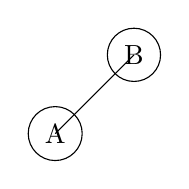
\begin{tikzpicture} \draw
  (1,1) node[circle, draw]{A} --
  (2,2) node[circle, draw]{B};
\end{tikzpicture}
\end{lstlisting}

\includesvg{/Users/mahmooz/brain/out/JuXxvo}\\[0pt]

to get a more "proper" result we use the \texttt{anchor} argument\\[0pt]

\begin{lstlisting}[language={[LaTeX]TeX},label= ,caption= ,captionpos=b,numbers=none]
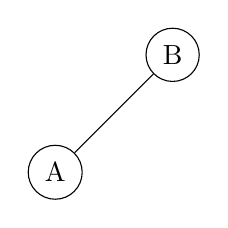
\begin{tikzpicture} \draw
  (1,1) node[anchor=north east, circle, draw]{A} --
  (2,2) node[anchor=south west, circle, draw]{B};
\end{tikzpicture}
\end{lstlisting}

\includesvg{/Users/mahmooz/brain/out/fwDlQd}\\[0pt]

\begin{lstlisting}[language={[LaTeX]TeX},label= ,caption= ,captionpos=b,numbers=none]
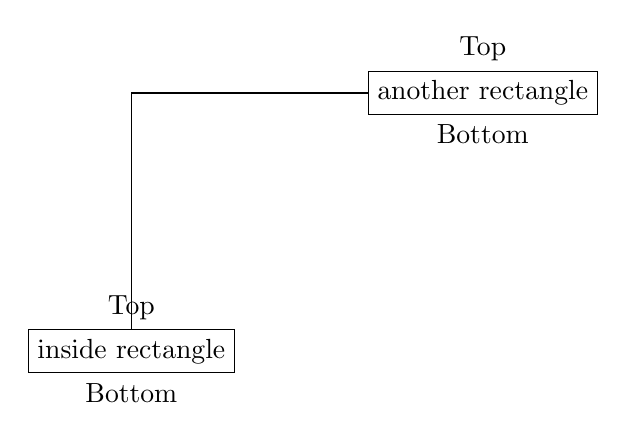
\begin{tikzpicture} \draw
  (0,0) node[anchor=north, rectangle, draw, label=above:Top, label=below:Bottom]{inside rectangle} |-
  (3,3) node[anchor=west, rectangle, draw, label=above:Top, label=below:Bottom]{another rectangle};
\end{tikzpicture}
\end{lstlisting}

\includesvg{/Users/mahmooz/brain/out/vERNnP}\\[0pt]

\begin{lstlisting}[language={[LaTeX]TeX},label= ,caption= ,captionpos=b,numbers=none]
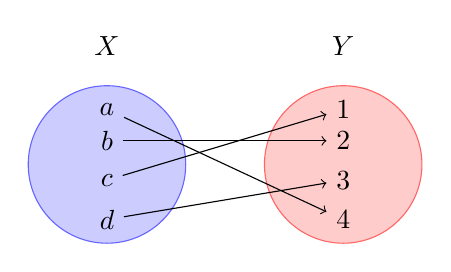
\begin{tikzpicture}
  % draw the sets
  \filldraw[fill=blue!20, draw=blue!60] (-1.5,0) circle (1cm);
  \filldraw[fill=red!20, draw=red!60] (1.5,0) circle (1cm);

  % the texts
  \node at (-1.5,1.5) {$X$};
  \node at (1.5,1.5) {$Y$};

  % the points in the sets (here I just create nodes to use them later on to position
  % the circles and the arrows
  \node (x1) at (-1.5,0.7) {$a$};
  \node (x2) at (-1.5,0.3) {$b$};
  \node (x3) at (-1.5,-0.2) {$c$};
  \node (x4) at (-1.5,-0.7) {$d$};
  \node (y1) at (1.5,0.7) {$1$};
  \node (y2) at (1.5,0.3) {$2$};
  \node (y3) at (1.5,-0.2) {$3$};
  \node (y4) at (1.5,-0.7) {$4$};

  % draw the arrows
  \draw[->] (x1) -- (y4);
  \draw[->] (x2) -- (y2);
  \draw[->] (x3) -- (y1);
  \draw[->] (x4) -- (y3);
\end{tikzpicture}
\end{lstlisting}

\includesvg{/Users/mahmooz/brain/out/BgY0KZ}\\[0pt]

\begin{lstlisting}[language={[LaTeX]TeX},label= ,caption= ,captionpos=b,numbers=none]
\begin{tikzpicture}[
    > = stealth, % arrow head style
    shorten > = 1pt, % don't touch arrow head to node
    auto,
    node distance = 1cm, % distance between nodes
    semithick % line style
  ]

  \tikzstyle{every state}=[
    draw = black,
    thin,
    fill = cyan!29,
    minimum size = 5mm
  ]

  \node[state] (a) {$a$};
  \node[state] (b)[below left=of a] {$b$};
  \node[state] (c)[below left=0.3cm and 0.3cm of b] {$c$};
  \node[state] (f)[below left=0.3cm and 0.3cm of c] {$f$};
  \node[state] (j)[below left=0.3cm and 0.3cm of f ] {$j$};
  \node[state] (d)[below left=0.3cm and 0.3cm of j] {$d$};
  \node[state] (i)[below left=0.3cm and 0.3cm of d] {$i$};

  \path[->] (a) edge node {} (b);
  \path[->] (b) edge node {} (c);
  \path[->] (c) edge node {} (f);
  \path[->] (f) edge node {} (j);
  \path[->] (j) edge node {} (d);
  \path[->] (d) edge node {} (i);
  \path[->] (b) edge[bend right=45, blue, very thick] node {} (j);
\end{tikzpicture}
\end{lstlisting}

\includesvg{/Users/mahmooz/brain/out/sP1ObG}\\[0pt]

\section{2d plots}
\label{sec:org04ec3f5}
you can play around with the parameters to see how they affect the drawing\\[0pt]
\begin{lstlisting}[language={[LaTeX]TeX},label= ,caption= ,captionpos=b,numbers=none]
\begin{tikzpicture}
  \draw[->] (-3, 0) -- (4.2, 0) node[right] {$x$};
  \draw[->] (0, -3) -- (0, 4.2) node[above] {$y$};
  \draw[scale=0.5, domain=-3:3, smooth, variable=\x, blue] plot ({\x}, {\x*\x});
  \draw[scale=0.5, domain=-3:3, smooth, variable=\y, red]  plot ({\y*\y}, {\y});
\end{tikzpicture}
\end{lstlisting}

\includesvg{/Users/mahmooz/brain/out/cdn8lr}\\[0pt]

\begin{lstlisting}[language={[LaTeX]TeX},label= ,caption= ,captionpos=b,numbers=none]
\begin{tikzpicture}
  % drawing the grid
  \draw[thick, color = gray, step = 1cm, dashed] (-1,-1) grid (5,5);
  \draw[->] (-2,0) -- (6,0) node[right]{$x$};
  \draw[->] (0,-2) -- (0,6) node[above]{$y$};

  % defining nodes
  \node (A) at (1,2);
  \node (B) at (2,4);
  \node (C) at (0,4);
  \node (D) at (5,2);
  \node (E) at (1.65, 3.35);

  % draw the lines
  \draw[red, thick, dashed] (A) -- (B);
  \draw[black, thick] (C) -- (D);

  % draw the points
  \draw[fill=orange] (E) circle (2pt) node[right] {E(1.65, 3.35)};
  \draw[fill=blue] (A) circle (2pt) node[below right] {A(1,2)};
  \draw[fill=blue] (B) circle (2pt) node[above left] {B(2,4)};
  \draw[fill=blue] (C) circle (2pt) node[below left] {C(0,4)};
  \draw[fill=blue] (D) circle (2pt) node[above right] {D(5,2)};
\end{tikzpicture}
\end{lstlisting}

\includesvg{/Users/mahmooz/brain/out/9DtrIs}\\[0pt]

\subsection{pgfplots}
\label{sec:org2f18aee}
you can use the \textbf{pgfplots} package which is written using \textbf{tikz} to make things easier, include it using:\\[0pt]
\begin{lstlisting}[language={[LaTeX]TeX},label= ,caption= ,captionpos=b,numbers=none]
\usepackage{pgfplots}
\end{lstlisting}
example usage:\\[0pt]
\begin{lstlisting}[language={[LaTeX]TeX},label= ,caption= ,captionpos=b,numbers=none]
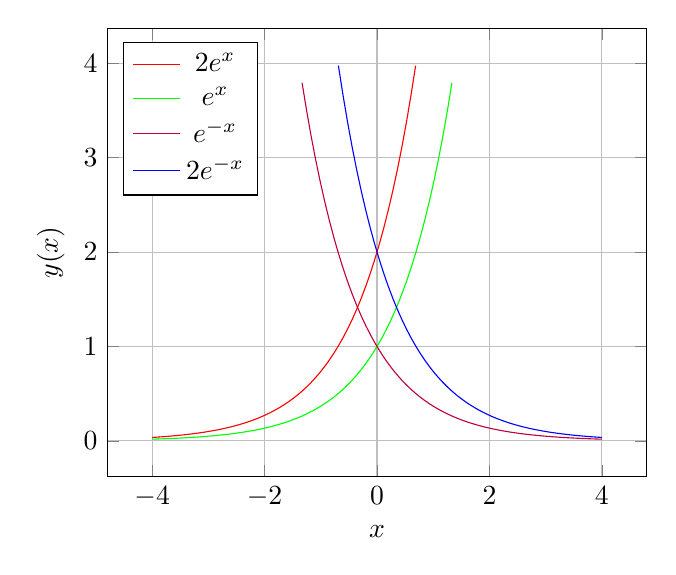
\begin{tikzpicture}
  \begin{axis}[domain=-4:4, samples=100, grid=major,
    restrict y to domain=0:4, xlabel=$x$, ylabel=$y(x)$, legend pos=north west]
    \addplot [color=red]    {2*exp(x)};
    \addplot [color=green]  {exp(x)};
    \addplot [color=purple] {exp(-x)};
    \addplot [color=blue]   {2*exp(-x)};

    \legend{$2e^x$, $e^x$, $e^{-x}$, $2e^{-x}$}
  \end{axis}
\end{tikzpicture}
\end{lstlisting}

\includesvg{/Users/mahmooz/brain/out/gSMHG5}\\[0pt]

\begin{lstlisting}[language={[LaTeX]TeX},label= ,caption= ,captionpos=b,numbers=none]
\usepgfplotslibrary{fillbetween}
\begin{tikzpicture}
  \begin{axis}[
    axis lines=middle, xlabel=$x$, ylabel=$y$,
    xmin=-3, xmax=3,
    ymin=-10, ymax=10,
    xtick distance=1, ytick distance=4]

    \addplot [domain=-2.5:2.5, samples=100, name path=f, thick, color=red!50]
    {3*x^3 - x^2 - 10*x};

    \addplot [domain=-2.5:2.5, samples=100, name path=g, thick, color=blue!50]
    {- x^2 + 2*x};

    \addplot[red!10, opacity=0.4] fill between[of=f and g, soft clip={domain=-2:2}];

    \node[color=red, font=\footnotesize] at (axis cs: -1.6,7) {$f(x)=3x^3 - x^2 - 10x$};
    \node[color=blue, font=\footnotesize] at (axis cs: 1.1,2.2) {$g(x)=- x^2 + 2x$};
  \end{axis}
\end{tikzpicture}
\end{lstlisting}

\includesvg{/Users/mahmooz/brain/out/7c8Bc5}\\[0pt]

\section{3d plots}
\label{sec:org336a9c7}
for 3d plots we use the package \texttt{tikz-3dplot}\\[0pt]
\begin{lstlisting}[language={[LaTeX]TeX},label= ,caption= ,captionpos=b,numbers=none]
\usepackage{tikz-3dplot}
\end{lstlisting}
we start with a simple 3d plot with 3 vectors\\[0pt]
\begin{lstlisting}[language={[LaTeX]TeX},label= ,caption= ,captionpos=b,numbers=none]
\tdplotsetmaincoords{70}{110}
\begin{tikzpicture}[tdplot_main_coords, scale=2]
  % draw main axes
  \draw[thick,->] (0,0,0) -- (1,0,0) node[anchor=north east]{$x$};
  \draw[thick,->] (0,0,0) -- (0,1,0) node[anchor=north west]{$y$};
  \draw[thick,->] (0,0,0) -- (0,0,1) node[anchor=south]{$z$};

  % draw the vector lines
  \draw[thick,color=blue,->] (0,0,0) -- (.7,.8,0) node[anchor=north]{$\vec{v_1}$};
  \draw[thick,color=blue,->] (0,0,0) -- (0,.7,.3) node[anchor=west]{$\vec{v_2}$};
  \draw[thick,color=blue,->] (0,0,0) -- (0,.2,.7) node[anchor=south]{$\vec{v_3}$};
\end{tikzpicture}
\end{lstlisting}

\includesvg{/Users/mahmooz/brain/out/EcA741}\\[0pt]

\begin{lstlisting}[language={[LaTeX]TeX},label= ,caption= ,captionpos=b,numbers=none]
\tdplotsetmaincoords{70}{130} % set initial 3d rotation
\begin{tikzpicture}[tdplot_main_coords, scale = 1]
  % draw the main axes
  \draw[thick, ->] (-2,0,0) -- (5,0,0) node[below left] {$x$};
  \draw[thick, ->] (0,-2,0) -- (0,5,0) node[below right] {$y$};
  \draw[thick, ->] (0,0,-2) -- (0,0,5) node[left] {$z$};

  \draw[thick, blue, dashed] (-1,4,8) -- (-5,-4,-4);
  \draw[thick, red, <->] (-4,-2,-1) -- (-2,2,5) node[midway, above, sloped, black] {vector};

  \filldraw[draw=black, fill=blue, opacity=0.3] (0,6,7) -- (-3,1,5) -- (-2,1,4) -- cycle;

  \draw[fill=black] (0,6,7) circle (2pt) node[below right] {(0,6,7)};
  \draw[fill=black] (-3,1,5) circle (2pt) node[above left] {(-3,1,5)};
  \draw[fill=black] (-2,1,4) circle (2pt) node[below left] {(-2,1,4)};
\end{tikzpicture}
\end{lstlisting}

\includesvg{/Users/mahmooz/brain/out/jAMOqE}\\[0pt]

\begin{lstlisting}[language={[LaTeX]TeX},label= ,caption= ,captionpos=b,numbers=none]
% set the plot display orientation
% syntax: \tdplotsetdisplay{\theta_d}{\phi_d}
\tdplotsetmaincoords{60}{110}

% define polar coordinates for some vector
% TODO: look into using 3d spherical coordinate system
\pgfmathsetmacro{\rvec}{.8}
\pgfmathsetmacro{\thetavec}{30}
\pgfmathsetmacro{\phivec}{60}

% use the tdplot_main_coords style to implement the display the coordinate transformation provided by 3dplot
\begin{tikzpicture}[scale=5,tdplot_main_coords]

  % set up some coordinates
  % -----------------------
  \node (O) at (0,0,0);

  % determine a coordinate (P) using (r,\theta,\phi) coordinates.  This command
  % also determines (Pxy), (Pxz), and (Pyz): the xy-, xz-, and yz-projections
  % of the point (P).
  % syntax: \tdplotsetcoord{Coordinate name without parentheses}{r}{\theta}{\phi}
  \tdplotsetcoord{P}{\rvec}{\thetavec}{\phivec}

  % draw the main coordinate system axes
  \draw[thick,->] (0,0,0) -- (1,0,0) node[anchor=north east]{$x$};
  \draw[thick,->] (0,0,0) -- (0,1,0) node[anchor=north west]{$y$};
  \draw[thick,->] (0,0,0) -- (0,0,1) node[anchor=south]{$z$};

  % draw a vector from origin to point (P) 
  \draw[-stealth,color=red] (O) -- (P);

  % draw projection on xy plane, and a connecting line
  \draw[dashed, color=red] (O) -- (Pxy);
  \draw[dashed, color=red] (P) -- (Pxy);

  % draw the angle \phi, and label it
  % syntax: \tdplotdrawarc[coordinate frame, draw options]{center point}{r}{angle}{label options}{label}
  \tdplotdrawarc{(O)}{0.2}{0}{\phivec}{anchor=north}{$\phi$}

  % set the rotated coordinate system so the x'-y' plane lies within the
  % "theta plane" of the main coordinate system
  % syntax: \tdplotsetthetaplanecoords{\phi}
  \tdplotsetthetaplanecoords{\phivec}

  % draw theta arc and label, using rotated coordinate system
  \tdplotdrawarc[tdplot_rotated_coords]{(0,0,0)}{0.5}{0}{\thetavec}{anchor=south west}{$\theta$}

  % draw some dashed arcs, demonstrating direct arc drawing
  \draw[dashed,tdplot_rotated_coords] (\rvec,0,0) arc (0:90:\rvec);
  \draw[dashed] (\rvec,0,0) arc (0:90:\rvec);

  % set the rotated coordinate definition within display using a translation
  % coordinate and Euler angles in the "z(\alpha)y(\beta)z(\gamma)" euler rotation convention
  % syntax: \tdplotsetrotatedcoords{\alpha}{\beta}{\gamma}
  \tdplotsetrotatedcoords{\phivec}{\thetavec}{0}

  % translate the rotated coordinate system
  % syntax: \tdplotsetrotatedcoordsorigin{point}
  \tdplotsetrotatedcoordsorigin{(P)}

  % use the tdplot_rotated_coords style to work in the rotated, translated coordinate frame
  \draw[thick,tdplot_rotated_coords,->] (0,0,0) -- (.5,0,0) node[anchor=north west]{$x'$};
  \draw[thick,tdplot_rotated_coords,->] (0,0,0) -- (0,.5,0) node[anchor=west]{$y'$};
  \draw[thick,tdplot_rotated_coords,->] (0,0,0) -- (0,0,.5) node[anchor=south]{$z'$};

  % WARNING:  coordinates defined by the \coordinate command (eg. (O), (P), etc.)
  % cannot be used in rotated coordinate frames.  Use only literal coordinates.  

  % draw some vector, and its projection, in the rotated coordinate frame
  \draw[-stealth,color=blue,tdplot_rotated_coords] (0,0,0) -- (.2,.2,.2);
  \draw[dashed,color=blue,tdplot_rotated_coords] (0,0,0) -- (.2,.2,0);
  \draw[dashed,color=blue,tdplot_rotated_coords] (.2,.2,0) -- (.2,.2,.2);

  % show its phi arc and label
  \tdplotdrawarc[tdplot_rotated_coords,color=blue]{(0,0,0)}{0.2}{0}{45}{anchor=north west,color=black}{$\phi'$}

  % change the rotated coordinate frame so that it lies in its theta plane.
  % Note that this overwrites the original rotated coordinate frame
  % syntax: \tdplotsetrotatedthetaplanecoords{\phi'}
  \tdplotsetrotatedthetaplanecoords{45}

  % draw theta arc and label
  \tdplotdrawarc[tdplot_rotated_coords,color=blue]{(0,0,0)}{0.2}{0}{55}{anchor=south west,color=black}{$\theta'$}
\end{tikzpicture}
\end{lstlisting}

\includesvg{/Users/mahmooz/brain/out/EUmDsX}\\[0pt]

\begin{lstlisting}[language={[LaTeX]TeX},label= ,caption= ,captionpos=b,numbers=none]
\begin{tikzpicture}[scale=3,line cap=round]
  \begin{scope}[rotate around y=45,rotate around z=30,canvas is zx plane at y=0]
    \draw [green!50!black, dashed, ultra thick] (-1,0) arc (180:360:1);
  \end{scope}

  \begin{scope}[canvas is zx plane at y=0]
    \draw [ultra thin, step = 0.25, lightgray] (-1,-1) grid (1,1);
    \draw [dashed, red] (225:1) -- (0,0) -- (135:1);
    \draw [green, ultra thick] (0, 0) circle (1);
    \foreach\i in{0,90}
    {
      \filldraw [fill= orange!20, draw = orange] (0,0) -- (\i:0.5) arc (\i:\i+45:0.5) -- cycle;
      \draw [->, orange, ultra thick] (0,0) -- (\i:1);
    }
    \node [anchor = north west] at (0, 1) {$\vec{i}$};
    \node [anchor = north]      at (1, 0) {$\vec{j}$};
  \end{scope}

  \begin{scope}[rotate around y=45,rotate around z=30]
    \draw [canvas is zx plane at y=0, green!50!black, ultra thick] (1, 0) arc (0:180:1);
    \foreach\i in {0,90}
    \filldraw [canvas is xy plane at z=0, fill=red!20, draw=red] (0,0) -- (\i-30:0.4) arc (\i-30:\i:0.4) -- cycle;
    \draw [->, red, ultra thick] (0,0,0) -- (1,0,0);
    \draw [->, red, ultra thick] (0,0,0) -- (0,1,0);
    \draw [->, red, ultra thick] (0,0,0) -- (0,0,1);
  \end{scope}

  \draw [->, orange, ultra thick] (0,0,0) -- (0,1,0) node[black, anchor=south east] at (0, 1, 0) {$\vec{z_0}$};
  \draw [canvas is zx plane at y=0.75, ->, blue] (0,-0.15) arc (-90:180:0.15);
  \node at (0.3,0.9) {$\dot{\Psi}\vec{z_0}$};

\end{tikzpicture}
\end{lstlisting}

\includesvg{/Users/mahmooz/brain/out/ggUg1y}\\[0pt]

\begin{lstlisting}[language={[LaTeX]TeX},label= ,caption= ,captionpos=b,numbers=none]
\tdplotsetmaincoords{80}{45}
\tdplotsetrotatedcoords{-90}{180}{-90}

%% style for surfaces
\tikzset{surface/.style={draw=blue!70!black, fill=blue!40!white, fill opacity=.6}}

%% macros to draw back and front of cones
%% optional first argument is styling; others are z, radius, side offset (in degrees)
\newcommand{\coneback}[4][]{
  %% start at the correct point on the circle, draw the arc, then draw to the origin of the diagram, then close the path
  \draw[canvas is xy plane at z=#2, #1] (45-#4:#3) arc (45-#4:225+#4:#3) -- (O) --cycle;
}
\newcommand{\conefront}[4][]{
  \draw[canvas is xy plane at z=#2, #1] (45-#4:#3) arc (45-#4:-135+#4:#3) -- (O) --cycle;
}
\begin{tikzpicture}[tdplot_main_coords]
  \coordinate (O) at (0,0,0);

  %% make sure to draw everything from back to front
  \coneback[surface]{-1.5}{2.5}{-15}
  \coneback[surface]{-3}{2}{-10}
  \draw (0,0,-5) -- (O);
  \conefront[surface]{-3}{2}{-10}
  \conefront[surface]{-1.5}{2.5}{-15}
  \filldraw[surface] circle (3);
  \draw[->] (-6,0,0) -- (6,0,0) node[right] {$x$};
  \draw[->] (0,-6,0) -- (0,6,0) node[right] {$y$};
  \coneback[surface]{1.5}{2.5}{15}
  \coneback[surface]{3}{2}{10}
  \draw[->] (O) -- (0,0,5) node[above] {$z$};
  \conefront[surface]{3}{2}{10}
  \conefront[surface]{1.5}{2.5}{15}
\end{tikzpicture}
\end{lstlisting}

\includesvg{/Users/mahmooz/brain/out/o79smS}\\[0pt]

\begin{lstlisting}[language={[LaTeX]TeX},label= ,caption= ,captionpos=b,numbers=none]
\newcommand{\ve}[1]{\ensuremath{\mathbf{#1}}}
\newcommand{\ud}[0]{\mathrm{d}}

\tikzset{
  vector/.style = {
    thick,
    > = stealth',
  },
  axis/.style = {
    very thin,
    > = stealth',
  },
}

\tdplotsetmaincoords{70}{120}
\tdplotsetrotatedcoords{90}{90}{90}
\begin{tikzpicture}[tdplot_main_coords,scale=0.5]
  \draw (0,0,0) -- ++(0,-2.3,0) node[left]{$-$};

  % draw a condensor plate
  \draw[fill=lightgray] (-1.5,0,-1.5)--(-1.5,0,1.5)--(1.5,0,1.5)--(1.5,0,-1.5)--cycle;
  \draw[fill=lightgray] (1.5,0,-1.5)--(1.5,-0.2,-1.5)--(1.5,-0.2,1.5)--(1.5,0,1.5)--cycle;
  \draw[fill=lightgray] (1.5,-0.2,1.5)--(-1.5,-0.2,1.5)--(-1.5,0,1.5)--(1.5,0,1.5)--cycle;

  \def\q{-2.3}

  % draw surface
  \draw (0,-0.5*\q,0) coordinate(R);
  \tdplotdrawarc[tdplot_rotated_coords,fill opacity=0.5,fill=lightgray!30,draw=black]{(R)}{3}{0}{360}{}{}
  \draw[tdplot_rotated_coords](R)++(-110:3) node[below left]{$S_2$};
  \draw[tdplot_rotated_coords](R)++(70:3) node[above]{$C$};

  % draw second condensor plate
  \draw[fill=lightgray] (-1.5,0-\q,-1.5)--(-1.5,0-\q,1.5)--(1.5,0-\q,1.5)--(1.5,0-\q,-1.5)--cycle;
  \draw[fill=lightgray] (1.5,0-\q,-1.5)--(1.5,-0.2-\q,-1.5)--(1.5,-0.2-\q,1.5)--(1.5,0-\q,1.5)--cycle;
  \draw[fill=lightgray] (1.5,-0.2-\q,1.5)--(-1.5,-0.2-\q,1.5)--(-1.5,0-\q,1.5)--(1.5,0-\q,1.5)--cycle;
  \draw (0,-\q,0)--++(0,2,0)node[right]{$+$};
\end{tikzpicture}%
\begin{tikzpicture}[tdplot_main_coords,scale=0.5]
  \tdplotsetrotatedcoords{90}{90}{90}%

  \draw (0,0,0)--++(0,-2.3,0)node[left]{$-$};

  % draw condensore plate
  \draw[fill=lightgray] (-1.5,0,-1.5)--(-1.5,0,1.5)--(1.5,0,1.5)--(1.5,0,-1.5)--cycle;
  \draw[fill=lightgray] (1.5,0,-1.5)--(1.5,-0.2,-1.5)--(1.5,-0.2,1.5)--(1.5,0,1.5)--cycle;
  \draw[fill=lightgray] (1.5,-0.2,1.5)--(-1.5,-0.2,1.5)--(-1.5,0,1.5)--(1.5,0,1.5)--cycle;

  % draw surface
  \def\q{-2.3}
  \def\R{3}
  \draw (0,-0.5*\q,0) coordinate(R);
  \tdplotdrawarc[tdplot_rotated_coords,fill=lightgray,fill opacity=0.5,draw=black]{(R)}{\R}{0}{360}{}{}
  \draw[tdplot_rotated_coords](R)++(-110:\R) node[below left]{$S_1$};
  \draw[tdplot_rotated_coords](R)++(70:\R) node[above]{$C$};
  \tdplotsetrotatedcoords{0}{70}{90}
  \draw[tdplot_rotated_coords](R)++(90:\R) coordinate (A) circle(0.5pt);
  \draw[tdplot_rotated_coords,fill opacity=0.5,fill=lightgray!30](A)arc(90:270:\R);
  \tdplotsetrotatedcoords{90}{90}{90}
  \tdplotdrawarc[tdplot_rotated_coords,fill=lightgray!10,draw=black]{(R)}{\R}{0}{360}{}{}
  \begin{scope}

    % draw condensor plate again, inside (clip outside)
    \clip[tdplot_rotated_coords] (R)++(0:\R) arc (0:360:\R);
    \draw[fill=lightgray] (-1.5,0,-1.5)--(-1.5,0,1.5)--(1.5,0,1.5)--(1.5,0,-1.5)--cycle;
    \draw[fill=lightgray] (1.5,0,-1.5)--(1.5,-0.2,-1.5)--(1.5,-0.2,1.5)--(1.5,0,1.5)--cycle;
    \draw[fill=lightgray] (1.5,-0.2,1.5)--(-1.5,-0.2,1.5)--(-1.5,0,1.5)--(1.5,0,1.5)--cycle;
  \end{scope}
  \draw[tdplot_rotated_coords] (R)++(0:\R) arc (0:360:\R);

  % draw second condensor plate
  \draw[fill=lightgray] (-1.5,0-\q,-1.5)--(-1.5,0-\q,1.5)--(1.5,0-\q,1.5)--(1.5,0-\q,-1.5)--cycle;
  \draw[fill=lightgray] (1.5,0-\q,-1.5)--(1.5,-0.2-\q,-1.5)--(1.5,-0.2-\q,1.5)--(1.5,0-\q,1.5)--cycle;
  \draw[fill=lightgray] (1.5,-0.2-\q,1.5)--(-1.5,-0.2-\q,1.5)--(-1.5,0-\q,1.5)--(1.5,0-\q,1.5)--cycle;
  \draw (0,-\q,0)--++(0,2,0)node[right]{$+$};
\end{tikzpicture}
\end{lstlisting}

\includesvg{/Users/mahmooz/brain/out/mq5YoS}\\[0pt]

\section{3d plots with pgfplots}
\label{sec:orgf1b6c85}

the \texttt{\textbackslash{}addplot3} makes drawing 3d graphics much easier, the syntax is simply \texttt{\textbackslash{}addplot \{<math expresion of f(x,y)>\};} which is a shorthand-hand equivalent for \texttt{\textbackslash{}addplot[<options>] expression \{<math expression of f(x,y)>\};}\\[0pt]

consider this example which plots \(f(x,y) = x^2 - y^2\):\\[0pt]

\begin{lstlisting}[language={[LaTeX]TeX},label= ,caption= ,captionpos=b,numbers=none]
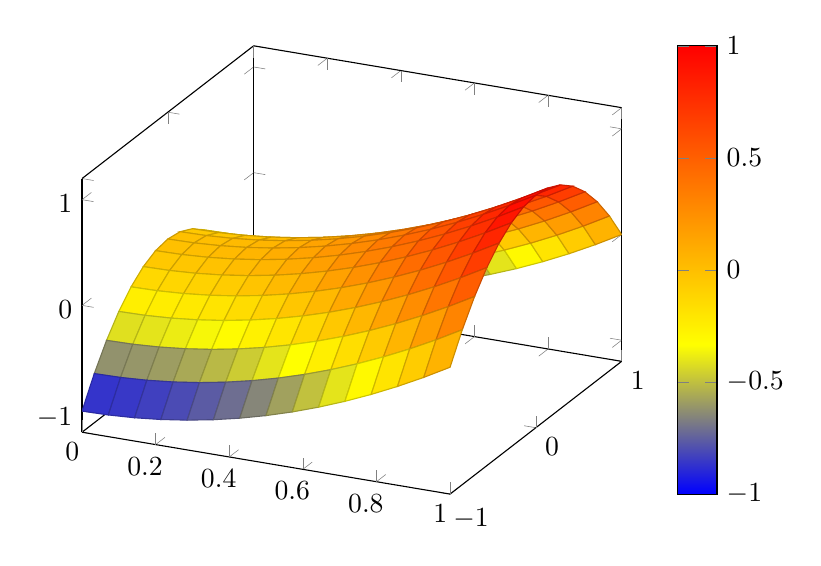
\begin{tikzpicture}
  \begin{axis}[colorbar]
    \addplot3 [
    surf,
    samples=15,
    domain=0:1,y domain=-1:1
    ] {x^2 - y^2};
  \end{axis}
\end{tikzpicture}
\end{lstlisting}

\includesvg{/Users/mahmooz/brain/out/4MXkkm}\\[0pt]

the \texttt{colorbar} argument passed to the \texttt{axis} environment simply generates the color bar on the right\\[0pt]

the \texttt{surf} argument passed to \texttt{axis} environment simply tells it to fill the gaps between the lines to form a solid surface\\[0pt]

a very useful variant of \texttt{\textbackslash{}addplot3} is one that takes 3 math expressions, one for each variable, the syntax is:\\[0pt]

\begin{lstlisting}[language={[LaTeX]TeX},label= ,caption= ,captionpos=b,numbers=none]
\addplot3[<options>] expression {<x expression>, <y expression>, <z expression>};
\end{lstlisting}

which for most purposes can be simplified to\\[0pt]

\begin{lstlisting}[language={[LaTeX]TeX},label= ,caption= ,captionpos=b,numbers=none]
\addplot3{<x expression>, <y expression>, <z expression>};
\end{lstlisting}

note that \texttt{\textbackslash{}addplot3(x,y,x\textasciicircum{}2)} is equivalent to \texttt{\textbackslash{}addplot\{x\textasciicircum{}2\}}\\[0pt]

consider the following examples\\[0pt]

\begin{lstlisting}[language={[LaTeX]TeX},label= ,caption= ,captionpos=b,numbers=none]
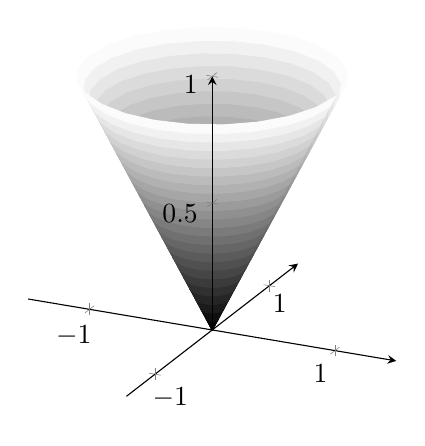
\begin{tikzpicture}
  \begin{axis}[
    axis lines=center,
    axis on top,
    domain=0:1,
    y domain=0:2*pi,
    xmin=-1.5, xmax=1.5,
    ymin=-1.5, ymax=1.5, zmin=0.0]
    \addplot3 [surf, colormap/blackwhite, shader=flat] ({x*cos(deg(y))},{x*sin(deg(y))},{x});
  \end{axis}
\end{tikzpicture}
\end{lstlisting}

\includesvg{/Users/mahmooz/brain/out/8mXtxD}\\[0pt]

\begin{lstlisting}[language={[LaTeX]TeX},label= ,caption= ,captionpos=b,numbers=none]
  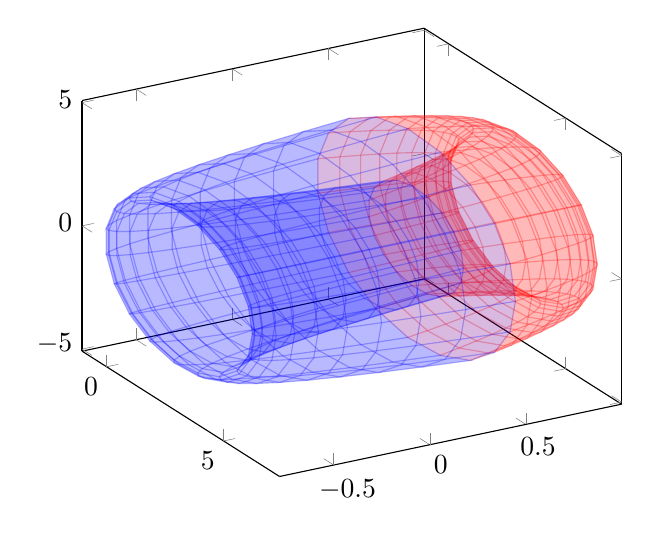
\begin{tikzpicture}
    \begin{axis}[view={60}{30}]
    \addplot3[surf,shader=flat,
      samples=20,
      color=red, opacity=0.15,
      domain=-1.11:1.11, y domain=0:2*pi,
      z buffer=sort
      ]
     ({(pi-x)*cos(deg(y))+pi}, {cos(deg(x))}, {(pi-x)*sin(deg(y))});
   \addplot3[surf,shader=flat,
     samples=20,
     color=blue, opacity=0.15,
     domain=-1.11:1.11, y domain=0:2*pi,
     z buffer=sort]
    ({(pi-x)*cos(deg(y))+pi}, {x*x-0.25*pi}, {(pi-x)*sin(deg(y))});
   \end{axis}
\end{tikzpicture}
\end{lstlisting}

\includesvg{/Users/mahmooz/brain/out/O4rtO3}\\[0pt]

\begin{lstlisting}[language={[LaTeX]TeX},label= ,caption= ,captionpos=b,numbers=none]
  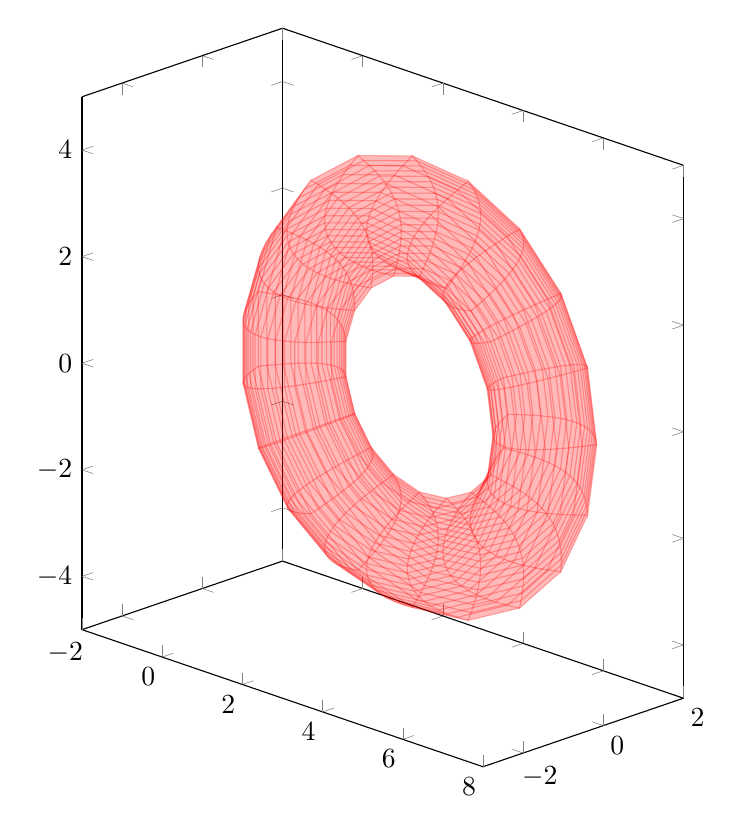
\begin{tikzpicture}
    \begin{axis}
    [   view={45}{20},
    unit vector ratio=1 1 1,
    xmin=-2, xmax=8,
    ymin=-3, ymax=2,
    zmin=-5, zmax=5,
    width=15cm,
    ]
    \addplot3[surf,shader=flat,
      samples=20,
      color=red, opacity=0.15,
      domain=-1.11:1.11, y domain=0:2*pi,
      z buffer=sort,
      ]
     ({(pi-x)*cos(deg(y))+pi}, {cos(deg(x))}, {(pi-x)*sin(deg(y))});
   \addplot3[surf,shader=flat,
     samples=20,
     color=red, opacity=0.15,
     domain=-1.11:1.11, y domain=0:2*pi,
     z buffer=sort]
    ({(pi-x)*cos(deg(y))+pi}, {x*x-0.25*pi}, {(pi-x)*sin(deg(y))});
   \end{axis}
\end{tikzpicture}
\end{lstlisting}

\includesvg{/Users/mahmooz/brain/out/cVNpiY}\\[0pt]

\begin{lstlisting}[language={[LaTeX]TeX},label= ,caption= ,captionpos=b,numbers=none]
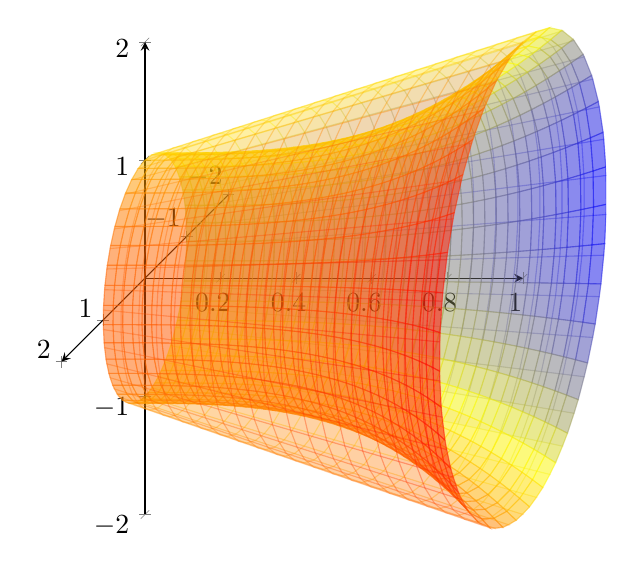
\begin{tikzpicture}
  \pgfmathsetmacro{\u}{1.5}
  \begin{axis}[set layers,
    x={(3.2*\u cm,0.0cm)}, 
    y={(0cm,\u cm)},
    z={(-\u*0.3535cm,-\u*0.3535cm)},  
    axis lines=center,
    xmin=0
    ]
    \addplot3[opacity=0.2,surf,shader=flat,on layer=axis background,
    samples=20,
    domain=0:1,y domain=pi:2*pi,
    z buffer=sort]
    (x,{(x + 1)*cos(deg(y))}, {(x+1) * sin(deg(y))});

    \addplot3[opacity=0.4,surf,shader=flat,on layer=main,
    samples=40,
    domain=0:1,y domain=0:2*pi,
    z buffer=sort]
    (x,{(x^3 + 1)*cos(deg(y))}, {(x^3 + 1) * sin(deg(y))});

    \addplot3[opacity=0.2,surf,shader=flat,on layer=axis foreground,
    samples=20,
    domain=0:1,y domain=0:pi,
    z buffer=sort]
    (x,{(x + 1)*cos(deg(y))}, {(x+1) * sin(deg(y))});
  \end{axis}
\end{tikzpicture}
\end{lstlisting}

\includesvg{/Users/mahmooz/brain/out/7XtVM6}\\[0pt]

\section{forest}
\label{sec:org854c873}

forest is a package used to draw "binary tree"-like diagrams\\[0pt]
it can be imported as:\\[0pt]

\begin{lstlisting}[language={[LaTeX]TeX},label= ,caption= ,captionpos=b,numbers=none]
\usepackage{forest}
\end{lstlisting}

\subsection{usage}
\label{sec:org3df7d9d}

\begin{lstlisting}[language={[LaTeX]TeX},label= ,caption= ,captionpos=b,numbers=none]
\begin{forest}
  [10
    [50
      [20]
      [30]
    ]
  ]
\end{forest}
\end{lstlisting}

\includesvg{/Users/mahmooz/brain/out/mQF4R6}\\[0pt]

what you put in the brackets is basically a \texttt{tikz} node and can take any shape, for example this is a binary tree with some basic math expressions and various shapes\\[0pt]

\begin{lstlisting}[language={[LaTeX]TeX},label= ,caption= ,captionpos=b,numbers=none]
\begin{forest}
  [$n$,rectangle,draw
    [$\dfrac{n}{3}$,circle,draw
      [$T\left(\dfrac{n}{9}\right)$,rectangle,draw]
      [$T\left(\dfrac{2n}{9}\right)$,circle,draw]
      [hello,circle,draw]
    ]
    [$\dfrac{2n}{3}$,circle,draw
      [$T\left(\dfrac{2n}{9}\right)$,ellipse,draw]
      [$T\left(\dfrac{4n}{9}\right)$,draw]
    ]
  ]
\end{forest}
\end{lstlisting}

\includesvg{/Users/mahmooz/brain/out/LOBRBL}\\[0pt]

to insert a node without drawing it so that you get the effect of an empty child but still have correct indentation for other children we use \texttt{[,phantom]} which is a node that gets inserted but not drawn, example:\\[0pt]

\begin{lstlisting}[language={[LaTeX]TeX},label= ,caption= ,captionpos=b,numbers=none]
\begin{forest}
  [$n$,rectangle,draw
    [$\dfrac{n}{3}$,circle,draw
      [,phantom]
      [$T\left(\dfrac{n}{9}\right)$,circle,draw]
    ]
    [$\dfrac{2n}{3}$,circle,draw
      [$T\left(\dfrac{2n}{9}\right)$,circle,draw]
      [$T\left(\dfrac{4n}{9}\right)$,circle,draw]
    ]
  ]
\end{forest}
\end{lstlisting}

\includesvg{/Users/mahmooz/brain/out/YQJ95R}\\[0pt]

you can treat the \texttt{forest} environment like \texttt{tikzpicture}, you can freely add more nodes and drawings, to use a node of \texttt{forest} as a tikz node you pass \texttt{name=<name>} to it, example:\\[0pt]

\begin{lstlisting}[language={[LaTeX]TeX},label= ,caption= ,captionpos=b,numbers=none]
\begin{forest}
  [5,circle,draw,name=root
    [3,circle,draw
      [2,circle,draw
        [1,circle,draw]
        [,phantom]
      ]
      [,phantom]
    ]
    [10,circle,draw
      [7,circle,draw]
      [18,circle,draw]
    ]
  ]
  \node (root_text) at (2,0) {root};
  \draw[->, blue] (root) -- (root_text);
\end{forest}
\end{lstlisting}

\includesvg{/Users/mahmooz/brain/out/bupAbG}\\[0pt]

a more advanced example:\\[0pt]
\begin{lstlisting}[language={[LaTeX]TeX},label= ,caption= ,captionpos=b,numbers=none]
\begin{forest}
  [5,circle,draw,name=root
    [3,circle,draw,name=n4
      [2,circle,draw,name=n5
        [1,circle,draw,name=n6]
        [,phantom]
      ]
      [,phantom]
    ]
    [10,circle,draw,name=n1
      [7,circle,draw,name=n2]
      [18,circle,draw,name=n3]
    ]
  ]
  % root text
  \node (root_text) at (2,0.5) {root};
  \draw[->, blue] (root) -- (root_text);
  % Tright
  \node (Tright_text) at (3,-3) {$T_{\text{right}(\text{root})}$};
  \node[draw=red, double, fit=(n1) (n3) (n2), inner sep=1ex, circle] (Tright) {};
  \draw[->, blue] (Tright) -- (Tright_text);
  % Tleft
  \node (Tleft_text) at (-4,-3) {$T_{\text{left}(\text{root})}$};
  \node[draw=green, double, fit=(n4) (n5) (n6), inner sep=1ex, ellipse] (Tleft) {};
  \draw[->, blue] (Tleft) -- (Tleft_text);
\end{forest}
\end{lstlisting}

\includesvg{/Users/mahmooz/brain/out/Yl6ICB}\\[0pt]

\begin{lstlisting}[language={[LaTeX]TeX},label= ,caption= ,captionpos=b,numbers=none]
\begin{forest}
  for tree={grow'=north}
  [A
    [B, edge label={node[midway,below,font=\scriptsize]{1}} [] [] [] [] [] [] [] [] [] []]
    [C, edge label={node[midway,below,font=\scriptsize]{2}} [] [] [] [] [] [] [] [] [] []]
  ]
\end{forest}
\end{lstlisting}

\includesvg{/Users/mahmooz/brain/out/KYyGNeh}\\[0pt]

\subsection{! \TeX{} capacity exceeded, sorry [save size=80000].}
\label{sec:orga3a1e9d}
to get over this increase the value of \texttt{save\_size} in \texttt{kpsewhich texmf.cnf}\\[0pt]
\section{calc projection}
\label{sec:org14805dd}
\url{https://tex.stackexchange.com/questions/25342/how-to-draw-orthogonal-vectors-using-tikz}\\[0pt]
the projection syntax from the calc library also takes an optional angle: (\((A)!(P)!90:(B)\)) is the projection of point (P) on the line from (A) to (B) after that line has been rotated 90 degrees around point (A). This makes it easy to draw the vector components:\\[0pt]
\section{animation}
\label{sec:org8cffcda}
\begin{lstlisting}[language={[LaTeX]TeX},label= ,caption= ,captionpos=b,numbers=none]
\foreach \v in {0,0.5,...,5}
{
\begin{tikzpicture}
  \draw[->] (-3, 0) -- (4.2, 0) node[right] {$x$};
  \draw[->] (0, -3) -- (0, 4.2) node[above] {$y$};
  \draw[scale=0.5, domain=-3:3, smooth, variable=\x, blue] plot ({\x+\v}, {\x*\x});
  \draw[scale=0.5, domain=-3:3, smooth, variable=\y, red]  plot ({\y*\y}, {\y+\v});
\end{tikzpicture}
}
\end{lstlisting}

\url{file:///Users/mahmooz/brain/out/e3xkrhv.gif}\\[0pt]
\end{document}